\chapter{Proposta}
\label{chp:capitulo4}

Este capítulo descreve a metodologia proposta para avaliar o impacto da engenharia de atributos físico-derivados na predição de endpoint em convertedores BOF. A tarefa é de \textbf{regressão supervisionada}: dados os parâmetros operacionais de entrada de uma corrida, predizer T\textsubscript{final}, C\textsubscript{final} e P\textsubscript{final} ao fim do sopro. A proposta se estrutura em quatro etapas — geração de dados, engenharia de atributos, treinamento comparativo e avaliação — executadas em três configurações experimentais distintas que permitem isolar os efeitos da escolha de arquitetura e do conjunto de features.

\begin{figure}[H]
\centering
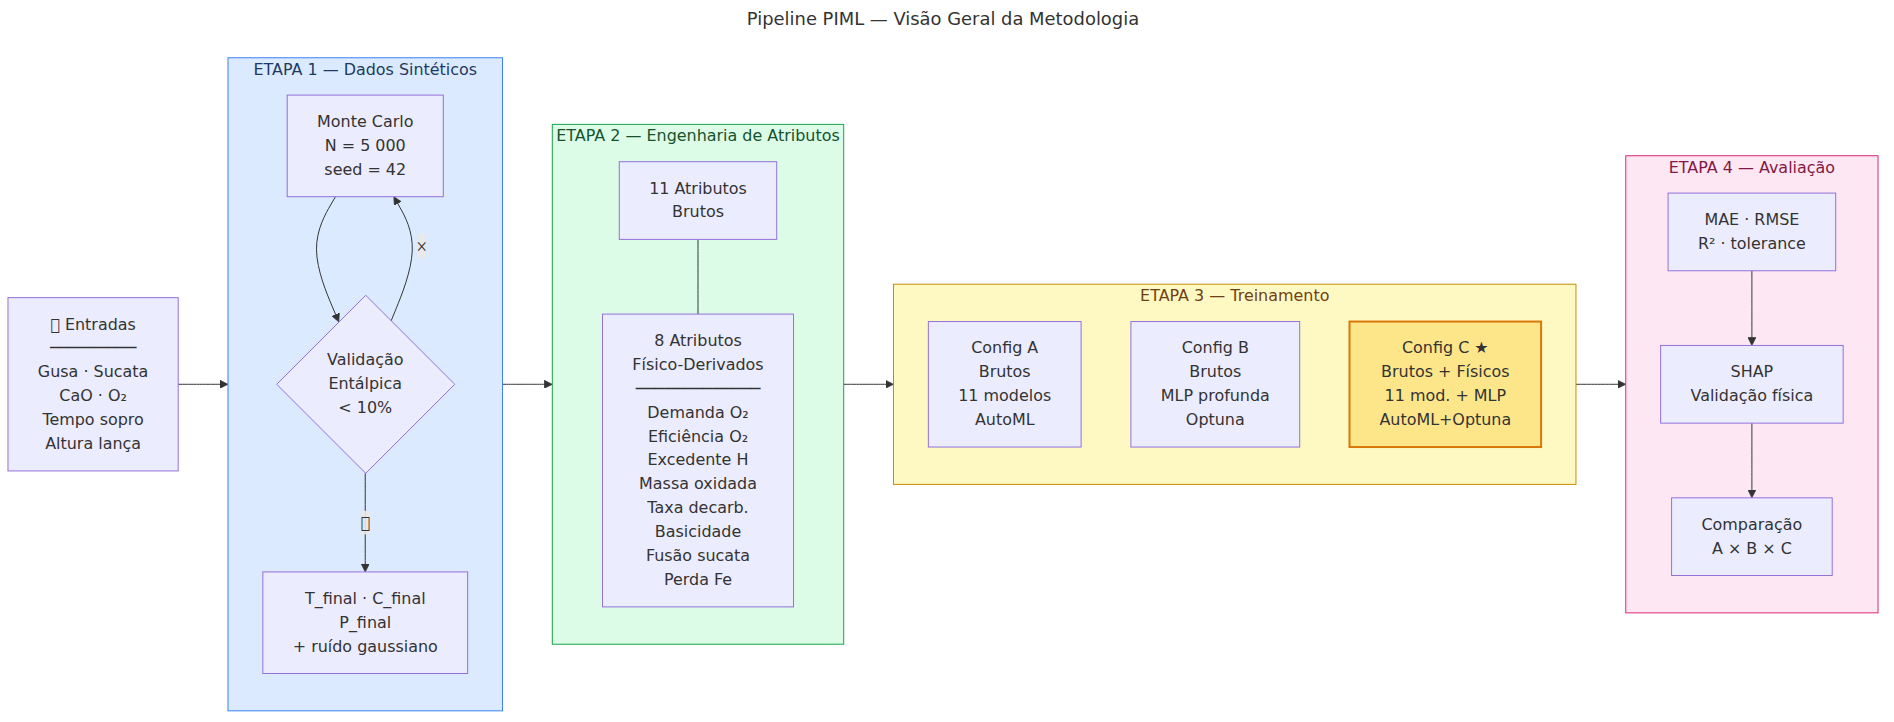
\includegraphics[width=0.88\textwidth,height=0.35\textheight,keepaspectratio]{Images/diagrams/01_piml_pipeline}
\caption{Visão geral do \textit{pipeline} metodológico proposto em quatro etapas: (1)~geração de dados sintéticos por Monte Carlo, (2)~engenharia de atributos físico-derivados, (3)~treinamento comparativo nas Configurações A, B e~C, e (4)~avaliação por métricas, análise de extrapolação e SHAP.}
\label{fig:piml-pipeline}
\end{figure}

%-------------------------------------------------------------------%
\section{Materiais}
\label{sec:materiais}

Os materiais computacionais necessários compreendem (i) o conjunto de dados sintético gerado especificamente para este trabalho, (ii) os modelos físico-químicos customizados que determinam os atributos físico-derivados e validam a plausibilidade das amostras, e (iii) as bibliotecas Python para AutoML, otimização de hiperparâmetros e interpretabilidade.

\subsection{Geração de Dados Sintéticos}
\label{subsec:dados-sinteticos}

Na ausência de dados reais de planta industrial, o conjunto de treinamento é gerado por amostragem de Monte Carlo\,\cite{buggineni2024synthetic,melo2024synthetic}. O procedimento adota $N = 10000$ amostras com semente \texttt{seed=42} para reprodutibilidade. Cada amostra é obtida por amostragem uniforme independente nas faixas físico-químicas da Tabela~\ref{tbl:ranges-sinteticos}, derivadas da literatura especializada em BOF\,\cite{xia2024dmpinn,chattopadhyay2022hybrid,bae2020bof}.

\textbf{Dados e constantes utilizados.} Nenhum dado industrial proprietário foi empregado neste trabalho. Todas as constantes físicas utilizadas --- capacidades caloríficas, entalpias de reação, razões estequiométricas e faixas operacionais --- são extraídas exclusivamente de literatura científica publicada\,\cite{cai2021heat,bae2020bof,chattopadhyay2022hybrid,xia2024dmpinn}. As referências específicas de cada constante constam nas equações da Tabela~\ref{tbl:features-fisicas} e nos comentários do código-fonte disponibilizado.

\begin{table}[H]
\centering
\caption{Faixas físico-químicas das 14 variáveis de entrada amostradas para geração de dados sintéticos. Duas delas ($S_\text{hm}$ e altura da lança) são amostradas e oferecidas como atributos aos modelos, mas não são lidas pelas equações físicas do gerador (Capítulo~\ref{chp:resultados}, Seção~\ref{sec:extrapolacao}).}
\label{tbl:ranges-sinteticos}
\small
\begin{tabular}{|p{4.2cm}|c|c|c|c|}
\hline
\textbf{Variável} & \textbf{Símbolo} & \textbf{Mín} & \textbf{Máx} & \textbf{Unidade} \\ \hline
Massa do gusa & $m_\text{hm}$ & 150 & 320 & t \\ \hline
Temperatura do gusa & $T_\text{hm}$ & 1250 & 1450 & °C \\ \hline
Carbono no gusa & $C_\text{hm}$ & 3{,}8 & 4{,}8 & \%~em~massa \\ \hline
Silício no gusa & $\text{Si}_\text{hm}$ & 0{,}3 & 1{,}2 & \%~em~massa \\ \hline
Manganês no gusa & $\text{Mn}_\text{hm}$ & 0{,}2 & 0{,}8 & \%~em~massa \\ \hline
Fósforo no gusa & $P_\text{hm}$ & 0{,}06 & 0{,}15 & \%~em~massa \\ \hline
Enxofre no gusa & $S_\text{hm}$ & 0{,}01 & 0{,}05 & \%~em~massa \\ \hline
Fração de sucata & $f_\text{scrap}$ & 0{,}10 & 0{,}30 & — \\ \hline
Carbono na sucata & $C_\text{scrap}$ & 0{,}05 & 0{,}25 & \%~em~massa \\ \hline
Adição de CaO & — & 15 & 60 & kg/t \\ \hline
Adição de MgO & — & 5 & 20 & kg/t \\ \hline
Fluxo de O$_2$ & — & 300 & 800 & Nm$^3$/min \\ \hline
Tempo de sopro & $t_\text{blow}$ & 12 & 22 & min \\ \hline
Altura da lança & — & 1{,}2 & 2{,}5 & m \\ \hline
\end{tabular}
\end{table}

Após a amostragem, cada instância é validada por dois critérios combinados por E-lógico — balanço entálpico e balanço de massa\,\cite{xia2024dmpinn,chattopadhyay2022hybrid} —, ambos exigidos para que a amostra seja aceita, embora, como discutido adiante, apenas o critério entálpico se mostre empiricamente restritivo dentro das faixas amostradas desta dissertação. O calor de entrada $Q_\text{in}$ inclui o calor sensível do gusa e o calor liberado pelas reações de oxidação dos elementos C, Si, Mn e P; o calor de saída $Q_\text{out}$ inclui o calor sensível do aço (base de massa do gusa, com a fusão da sucata contabilizada separadamente como o sorvedouro $Q_\text{scrap}$) e as perdas térmicas do processo, modeladas pela fração complementar $(1-\eta_\text{eff})$ da eficiência térmica específica da corrida (calibração e distribuição de $\eta_\text{eff}$ detalhadas na Seção~\ref{subsec:ameacas-validade}):

\begin{align}
Q_\text{in}  &= m_\text{hm}\,C_{p,\text{hm}}\,(T_\text{hm} - T_\text{ref}) + \sum_i \frac{m_\text{hm}\,x_i\,|\Delta H_i|}{M_i} \label{eq:q-in} \\
Q_\text{out} &= m_{\text{steel},\text{hm}}\,C_{p,\text{steel}}\,(T_\text{final} - T_\text{ref}) + Q_\text{scrap} + (1-\eta_\text{eff})\,Q_\text{in} \label{eq:q-out}
\end{align}

\noindent em que $C_{p,\text{hm}} = 0{,}82$\,kJ/(kg·°C), $C_{p,\text{steel}} = 0{,}75$\,kJ/(kg·°C), $T_\text{ref} = 25$\,°C e $\Delta H_i$ são as entalpias de oxidação de cada elemento\,\cite{chattopadhyay2022hybrid,madhavan2020heatbalance}; $m_{\text{steel},\text{hm}}$ é a massa de aço com base apenas no gusa; $Q_\text{scrap} = m_\text{scrap}\,C_{p,\text{scrap}}\,(T_\text{fusão} - T_\text{ref})$, com $C_{p,\text{scrap}} = 0{,}68$\,kJ/(kg·°C) e $T_\text{fusão} = 1500$\,°C, é o calor absorvido na fusão da sucata. Por construção, $Q_\text{out} \equiv Q_\text{in}$ quando $T_\text{final}$ assume seu valor físico antes da adição de ruído de medição e do truncamento de faixa (Equação~\ref{eq:q-out} é algebricamente derivada da mesma relação usada para gerar $T_\text{final}$, Seção~\ref{subsec:ameacas-validade}) — o critério de rejeição, portanto, não testa a física em si, mas se o ruído e o truncamento aplicados após o cálculo físico produziram uma amostra implausível. O critério de balanço de massa exige que a fração de massa não-oxidada (\textit{yield}) do carregamento total exceda 80\,\%\,\cite{chattopadhyay2022hybrid}. Dentro das faixas físico-químicas amostradas (Tabela~\ref{tbl:ranges-sinteticos}), o pior caso teórico de oxidação produz \textit{yield} $\approx 94{,}6\,\%$ — acima do limiar para qualquer combinação válida de entradas —, de modo que, na prática, nenhuma rejeição do dataset gerado é atribuível a este critério; ele é mantido como salvaguarda caso as faixas de amostragem sejam estendidas em trabalhos futuros, não como filtro ativo nesta versão do dataset. Amostras que violam qualquer um dos critérios

\begin{equation}
\frac{|Q_\text{in} - Q_\text{out}|}{Q_\text{in}} < 0{,}10 \label{eq:criterio-entalpico}
\end{equation}

\noindent são descartadas e substituídas por novas amostras até atingir $N = 10000$ instâncias válidas. Das 10.521 amostras efetivamente avaliadas pelos critérios até completar as 10.000 instâncias válidas, 521 ($5{,}0\,\%$) foram rejeitadas — na prática, integralmente pelo critério entálpico (ver acima) — taxa compatível com o efeito esperado do ruído gaussiano pós-cálculo sobre um balanço que é exato por construção antes da adição de ruído. As variáveis-alvo — T\textsubscript{final} (1620–1700\,°C), C\textsubscript{final} (0{,}02–0{,}10\,\%~em~massa) e P\textsubscript{final} (0{,}005–0{,}025\,\%~em~massa) — são calculadas por um modelo físico simplificado com adição de ruído gaussiano calibrado ($\sigma_T = 5$\,°C, $\sigma_C = 0{,}003$\,\%~em~massa, $\sigma_P = 0{,}001$\,\%~em~massa), representando a incerteza combinada de sensor e processo\,\cite{xia2024dmpinn,bae2020bof}. Os valores foram calibrados a partir de especificações de instrumentação BOF reportadas na literatura: sistemas de medição de temperatura por sub-lança apresentam incerteza típica de $\pm$3–8\,°C\,\cite{chattopadhyay2022hybrid,zhou2024bof}; analisadores de carbono em aço líquido operam com precisão de $\pm$0{,}002–0{,}005\,\%~em~massa; e o teor de fósforo, medido por espectrometria de emissão óptica em amostras de escória, apresenta incerteza de $\pm$0{,}001–0{,}002\,\%~em~massa\,\cite{bae2020bof,chattopadhyay2022hybrid}. Os valores adotados situam-se no limite inferior dessas faixas, representando condições instrumentais favoráveis compatíveis com instalações modernas de BOF. As três variáveis-alvo são truncadas em seus limites físicos (acima) após o cálculo e a adição de ruído; no dataset final, uma fração relevante das amostras satura em um dos limites --- $40{,}5\,\%$ para $T_\text{final}$, $35{,}2\,\%$ para $[\text{C}]_\text{final}$ e $13{,}4\,\%$ para $[\text{P}]_\text{final}$ --- refletindo que a combinação das faixas de amostragem de entrada (Tabela~\ref{tbl:ranges-sinteticos}) com a variabilidade estocástica por corrida (§\,\ref{subsec:ameacas-validade}) produz, antes do truncamento, uma distribuição mais larga que a faixa fisicamente plausível adotada para cada alvo. Essa censura nos limites tem implicação direta na leitura de $R^2$ no Capítulo~\ref{chp:resultados}: amostras saturadas são, em média, mais previsíveis (a saturação por si só reduz a variância a explicar), de modo que o $R^2$ calculado sobre a amostra completa é sistematicamente mais otimista que o calculado apenas sobre amostras não saturadas.


\begin{figure}[H]
\centering
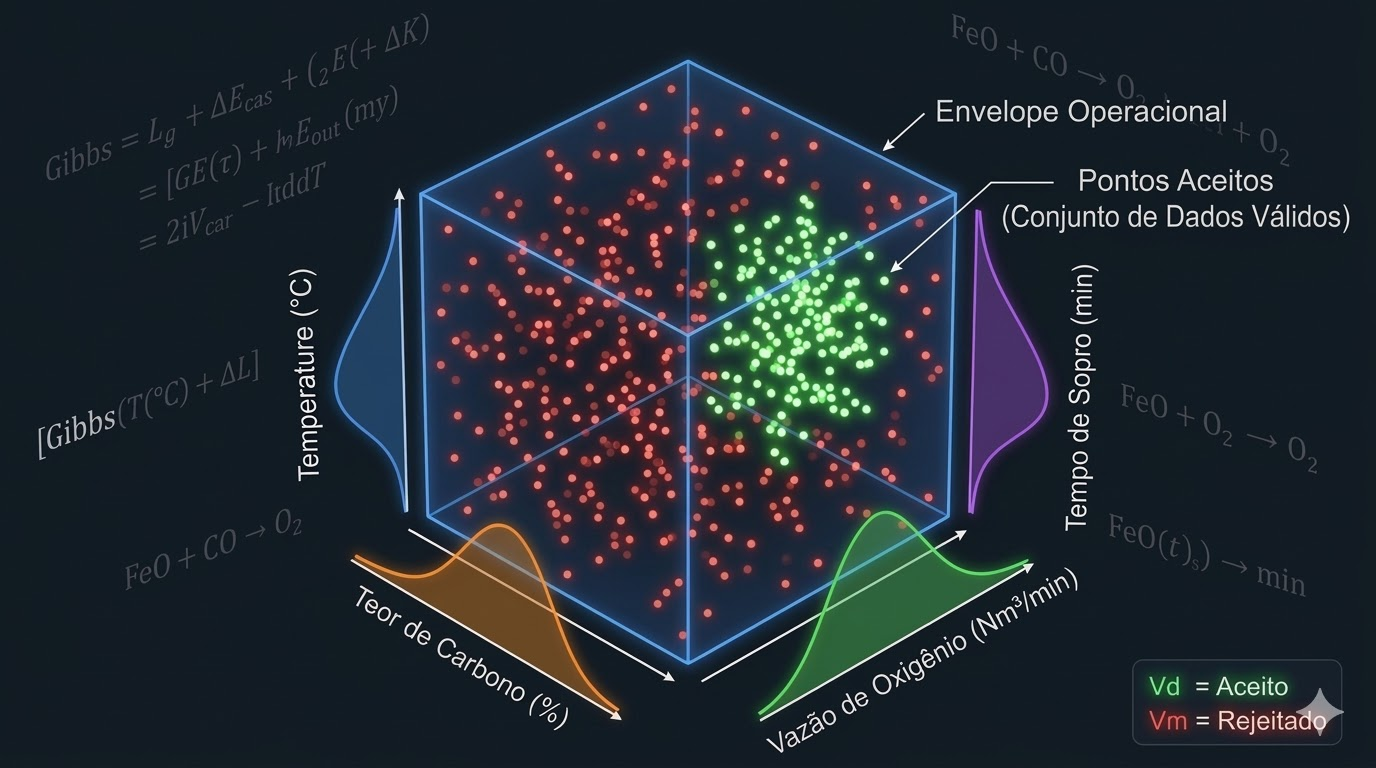
\includegraphics[width=0.60\textwidth]{Images/MonteCarlo}
\caption{Envelope operacional tridimensional da amostragem Monte Carlo para o dataset BOF sintético. Pontos verdes representam amostras aceitas (fisicamente válidas); pontos vermelhos, amostras rejeitadas por violação do critério de balanço entálpico (Equação~\ref{eq:criterio-entalpico}). Ilustração gerada com auxílio de inteligência artificial (Nano Banana Pro~3).}
\label{fig:monte-carlo-envelope}
\end{figure}

\begin{figure}[htbp]
\centering
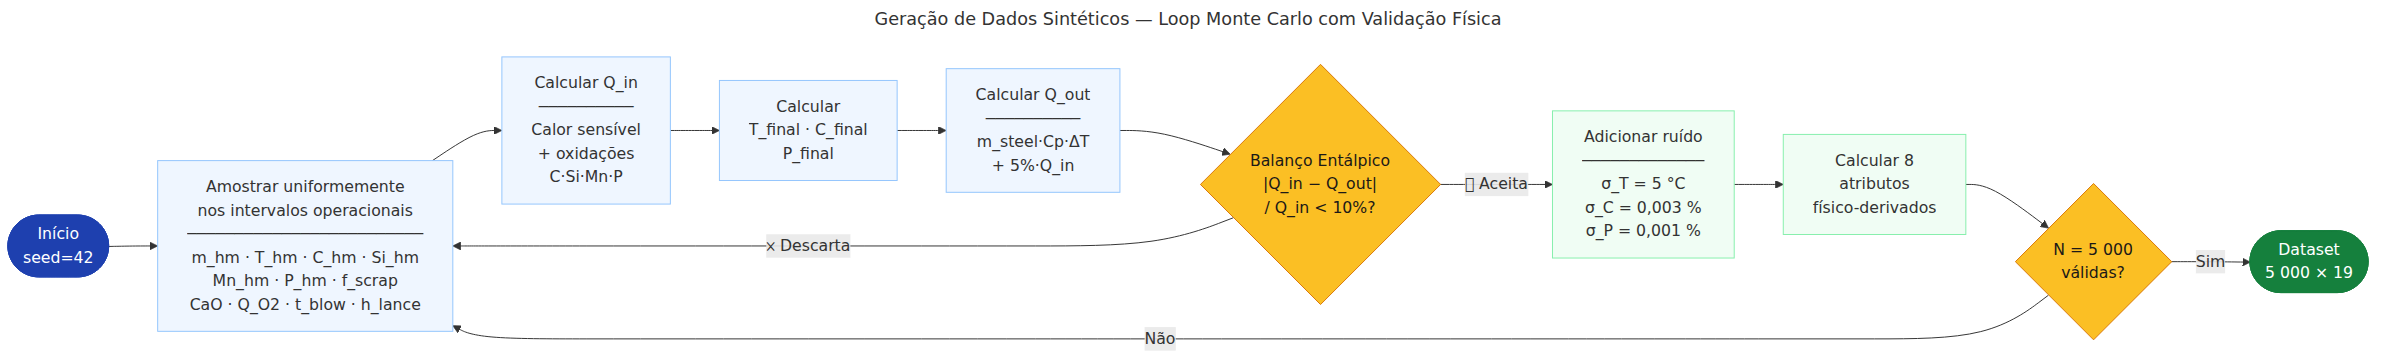
\includegraphics[width=0.88\textwidth,height=0.22\textheight,keepaspectratio]{Images/diagrams/02_monte_carlo_loop}
\caption{Fluxograma do loop de geração de dados sintéticos por Monte Carlo com validação de balanço entálpico. Amostras que violam o critério da Equação~\ref{eq:criterio-entalpico} são descartadas e o processo é repetido até $N = 10000$ instâncias válidas.}
\label{fig:monte-carlo-loop}
\end{figure}

\subsection{Atributos Físico-Derivados}
\label{subsec:feature-engineering}

A partir das variáveis brutas de cada instância, são calculados oito atributos físico-derivados com significado termodinâmico e estequiométrico direto\,\cite{chattopadhyay2022hybrid,shao2024hybrid,willard2020integrating}. Esses atributos condensam relações não-lineares entre variáveis de entrada que algoritmos puramente orientados a dados precisariam descobrir implicitamente a partir de exemplos\,\cite{cuomo2022physics}. A Tabela~\ref{tbl:features-fisicas} descreve cada atributo.

\begin{table}[H]
\centering
\caption{Atributos físico-derivados incorporados na Configuração~C}
\label{tbl:features-fisicas}
\small
\begin{tabular}{|p{3.8cm}|p{5.5cm}|p{4.7cm}|}
\hline
\textbf{Atributo} & \textbf{Fórmula (simplificada)} & \textbf{Significado físico} \\ \hline
\texttt{theo\_o2\_demand} & $m_\text{hm} \sum_i x_i \cdot r_i$ & O$_2$ mínimo para oxidar todas as impurezas \\ \hline
\texttt{o2\_efficiency} & $\text{theo\_o2} / (Q_{O_2} \cdot t_\text{blow})$ & Taxa de utilização do O$_2$ soprado \\ \hline
\texttt{enthalpy\_surplus} & $Q_\text{in} - Q_\text{out,scrap}$ & Energia disponível para fundir sucata \\ \hline
\texttt{total\_oxidized\_mass} & $\sum_i \Delta x_i \cdot m_\text{hm}$ & Massa total removida do banho \\ \hline
\texttt{decarb\_rate} & $C_\text{hm} / t_\text{blow}$ & Demanda teórica de descarburação por minuto de sopro \\ \hline
\texttt{slag\_basicity} & $\text{CaO} / (\text{Si}_\text{hm} \cdot m_\text{hm} \cdot f)$ & Capacidade de remoção de fósforo \\ \hline
\texttt{scrap\_melt\_capacity} & $\text{enthalpy\_surplus} / (C_{p,\text{scrap}} \cdot \Delta T)$ & Máximo de sucata fundível \\ \hline
\texttt{fe\_oxidation\_loss} & $(O_{2,\text{real}} - \text{theo\_o2}) \cdot r_\text{Fe}$ & Ferro perdido para a escória \\ \hline
\end{tabular}
\end{table}

\begin{figure}[H]
\centering
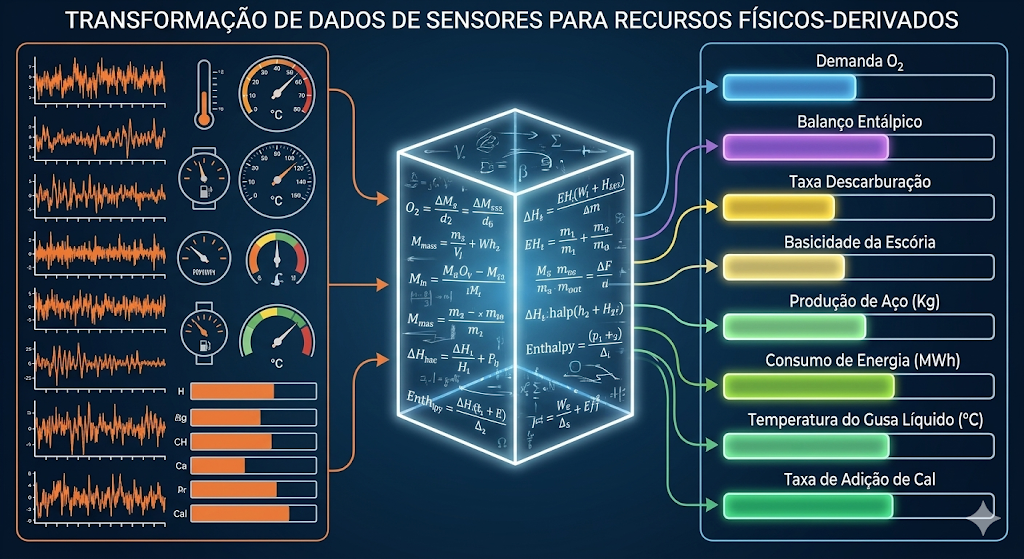
\includegraphics[width=0.65\textwidth]{Images/Raw_to_FeatureEngineered}
\caption{Transformação de dados brutos de sensores nos oito atributos físico-derivados: sinais de termopares, medidores de fluxo e espectrômetros (esquerda) são processados por balanços de massa e energia (centro), gerando grandezas com significado termodinâmico direto como demanda de O\textsubscript{2}, balanço entálpico, taxa de descarburação e basicidade da escória (direita). Ilustração gerada com auxílio de inteligência artificial (Nano Banana Pro~3).}
\label{fig:feature-engineering}
\end{figure}

%-------------------------------------------------------------------%
\section{Métodos}
\label{sec:metodos}

\subsection{Configurações Experimentais}
\label{subsec:configuracoes}

A metodologia proposta adota três configurações experimentais, permitindo isolar os efeitos da escolha de modelo e do conjunto de atributos\,\cite{zhou2024bof,he2021automl}:

\begin{itemize}
  \item \textbf{Config A — Linha de base}: modelos treinados exclusivamente com as variáveis brutas da Tabela~\ref{tbl:ranges-sinteticos}, com hiperparâmetros otimizados via Optuna\,\cite{akiba2019optuna} sobre o conjunto pré-definido de onze modelos da Tabela~\ref{tbl:modelos-ml} (implementação direta, sem uso de um framework de AutoML de portfólio como PyCaret ou Auto-sklearn\,\cite{he2021automl} — ver §\,\ref{subsec:otimizacao-treinamento}). Serve como referência para avaliar o ganho de desempenho das demais configurações.
  \item \textbf{Config B — Aprendizado profundo}: somente MLP com busca de arquitetura profunda via Optuna\,\cite{goodfellow2016deep,kingma2015adam}, treinada nas variáveis brutas. Isola o efeito da capacidade de representação da rede neural frente ao conjunto de modelos da Config~A.
  \item \textbf{Config C — Físico-informada}: mesmo conjunto completo de modelos da Config~A mais a MLP da Config~B, treinados no conjunto de variáveis brutas \emph{acrescido} dos oito atributos físico-derivados da Tabela~\ref{tbl:features-fisicas}\,\cite{xia2024dmpinn,willard2020integrating}. A comparação A$\times$C isola o efeito dos atributos físicos; A$\times$B isola o efeito da profundidade da rede; B$\times$C testa ambos simultaneamente.
\end{itemize}

\begin{figure}[H]
\centering
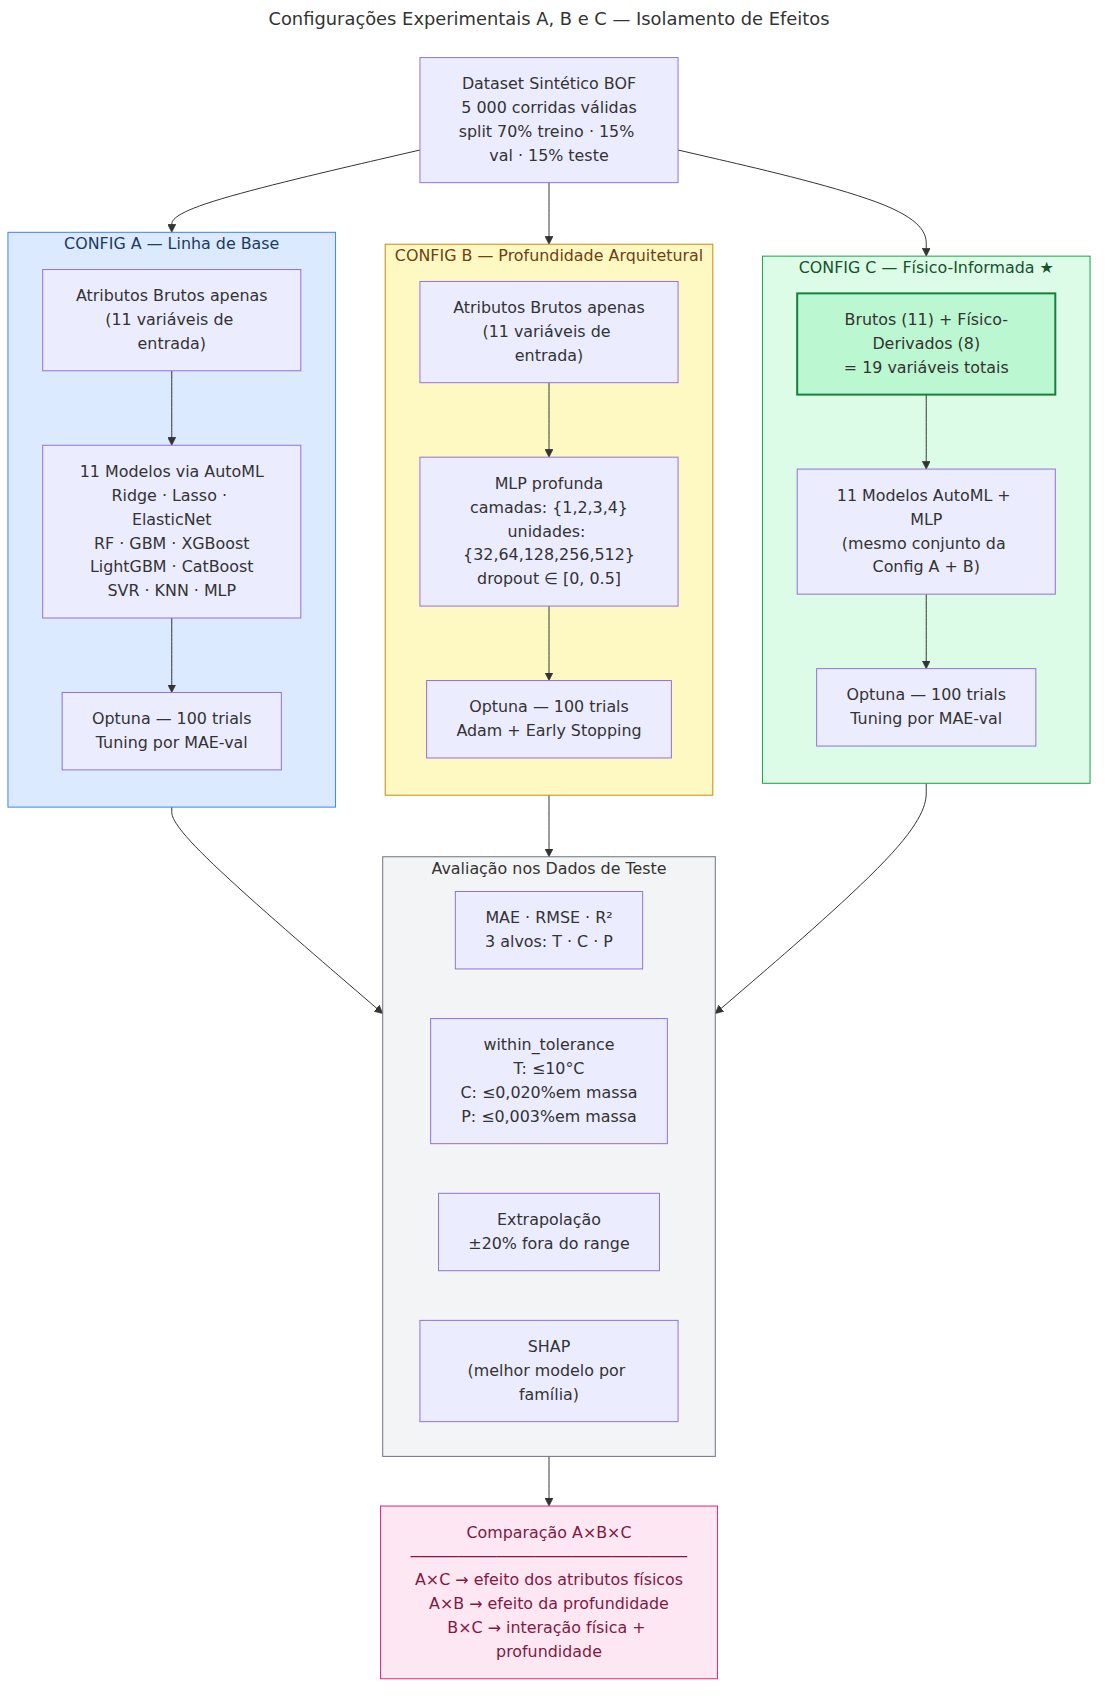
\includegraphics[width=0.80\textwidth,height=0.48\textheight,keepaspectratio]{Images/diagrams/04_experimental_configs}
\caption{Configurações experimentais A, B e~C: a Config~A serve como linha de base com atributos brutos; a Config~B isola o efeito da profundidade arquitetural da MLP; a Config~C incorpora os oito atributos físico-derivados ao mesmo conjunto de modelos da Config~A. A comparação cruzada A$\times$C, A$\times$B e B$\times$C permite isolar os efeitos de arquitetura e engenharia de atributos.}
\label{fig:experimental-configs}
\end{figure}

\begin{figure}[H]
\centering
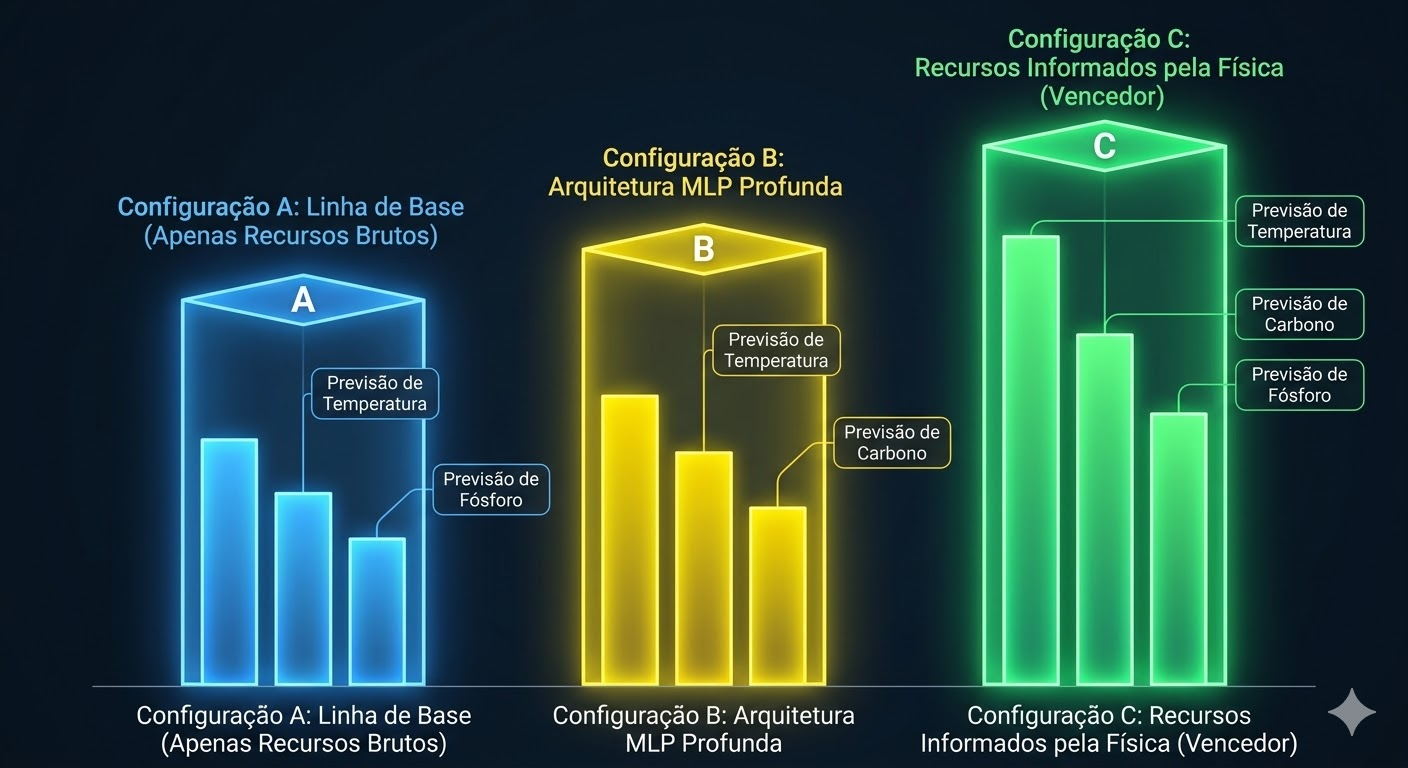
\includegraphics[width=0.60\textwidth]{Images/Configs}
\caption{Representação conceitual da hipótese de trabalho \emph{a priori}: a Config~C (físico-informada) melhoraria o desempenho nos três alvos frente às configurações A e~B. Os resultados reais (Capítulo~\ref{chp:resultados}) confirmam esse ganho para $[\text{C}]_\text{final}$ e $[\text{P}]_\text{final}$, mas não para $T_\text{final}$. Ilustração gerada com auxílio de inteligência artificial (Nano Banana Pro~3).}
\label{fig:configs-comparison}
\end{figure}

\subsection{Modelos de Regressão Supervisionada}
\label{subsec:modelos}

O conjunto de modelos avaliados nas Configs A e C é apresentado na Tabela~\ref{tbl:modelos-ml}. A seleção cobre as principais famílias de algoritmos de ML documentadas na literatura de predição de processos industriais\,\cite{zhou2024bof,chattopadhyay2022hybrid}.

\begin{table}[H]
\centering
\caption{Modelos de regressão supervisionada avaliados nas Configurações~A e~C}
\label{tbl:modelos-ml}
\small
\begin{tabular}{|p{3.0cm}|p{2.8cm}|p{8.2cm}|}
\hline
\textbf{Modelo} & \textbf{Família} & \textbf{Justificativa e referência} \\ \hline
Ridge & Linear L2 & Regularização $\ell_2$ reduz variância em espaços de alta dimensão\,\cite{hoerl1970ridge} \\ \hline
Lasso & Linear L1 & Regularização $\ell_1$ induz esparsidade e seleção implícita de atributos\,\cite{tibshirani1996regression} \\ \hline
ElasticNet & Linear L1+L2 & Combina vantagens de Ridge e Lasso; eficaz quando features são correlacionadas\,\cite{zou2005regularization} \\ \hline
Random Forest & Ensemble bagging & Boa capacidade de capturar não-linearidades sem overfitting excessivo\,\cite{breiman2001randomforests}; amplamente avaliado em predição de endpoint BOF\,\cite{zhou2024bof,chattopadhyay2022hybrid} \\ \hline
Gradient Boosting & Ensemble boosting & Boosting gradiente para regressão\,\cite{friedman2001greedy}, amplamente adotado em problemas industriais\,\cite{zhou2024bof} \\ \hline
XGBoost & Boosting otimizado & Regularização adicional e desempenho computacional superior a GBM padrão\,\cite{chen2016xgboost}; avaliado em predição de endpoint BOF\,\cite{zhou2024bof} \\ \hline
LightGBM & Boosting eficiente & Crescimento por folha com baixo consumo de memória para datasets médios\,\cite{ke2017lightgbm}; avaliado em predição de endpoint BOF\,\cite{zhou2024bof} \\ \hline
CatBoost & Boosting robusto & Tratamento nativo de variáveis categóricas; robusto a hiperparâmetros padrão\,\cite{prokhorenkova2018catboost}; avaliado em predição de endpoint BOF\,\cite{zhou2024bof} \\ \hline
SVR & Kernel & Eficaz em datasets de tamanho moderado com margem de insensibilidade ao ruído\,\cite{widodo2007svm} \\ \hline
KNN & Baseado em instâncias & Referência simples não-paramétrica; útil para verificar localidade do problema\,\cite{bishop2006prml} \\ \hline
MLP & Rede neural & Capacidade de aproximação universal; base da Config~B com busca profunda de arquitetura\,\cite{goodfellow2016deep} \\ \hline
\end{tabular}
\end{table}

\subsection{Protocolo de Treinamento e Avaliação}
\label{subsec:protocolo}

O protocolo de treinamento é idêntico para todas as configurações, garantindo comparabilidade. O dataset é dividido aleatoriamente em 70\,\% treino, 15\,\% validação e 15\,\% teste (seed=42)\,\cite{kohavi1995study} — sem estratificação, uma vez que os três alvos são variáveis contínuas e a amostragem de entrada já é aproximadamente uniforme (§\,\ref{subsec:preprocessamento}). A otimização de hiperparâmetros é realizada com o framework Optuna\,\cite{akiba2019optuna} sobre um conjunto pré-definido de modelos (Tabela~\ref{tbl:modelos-ml}), adotando 20 \textit{trials} por modelo por alvo — valor selecionado para equilibrar qualidade de busca e custo computacional com $N = 10000$ amostras; benchmarks em regressão tabular indicam retornos decrescentes além de 20--30 avaliações para espaços de hiperparâmetros de dimensão moderada\,\cite{he2021automl} —, amostrador TPE (\textit{Tree-structured Parzen Estimator})\,\cite{bergstra2011tpe} e objetivo de minimizar o MAE médio de validação cruzada com $k = 3$ folds sobre o conjunto de treino\,\cite{kohavi1995study} — valor de $k$ reduzido de 5 para conter o custo computacional total do protocolo (72 combinações modelo$\times$config$\times$alvo, 20 \textit{trials} cada). A partição de validação (15\,\%) é reservada na divisão do dataset mas, na versão atual do pipeline, não é consumida por nenhuma etapa do protocolo — nem o \textit{tuning} (que usa validação cruzada sobre o treino), nem a seleção de modelo final, nem as métricas reportadas neste capítulo, que se baseiam exclusivamente no conjunto de teste; a partição permanece disponível para uso futuro como critério de parada antecipada ou seleção hold-out independente da validação cruzada.

Para a Config~B, a busca de arquitetura da MLP percorre: número de camadas ocultas $\in \{1, 2, 3, 4\}$, unidades por camada $\in [32, 512]$ (inteiro, busca contínua) e taxa de aprendizado $\in [10^{-4}; 10^{-2}]$ — faixas consistentes com práticas consolidadas para redes neurais em regressão de processos industriais\,\cite{goodfellow2016deep,chattopadhyay2022hybrid} —, com regularização $\ell_2$ (\texttt{alpha})\,\cite{hoerl1970ridge}, otimizador Adam\,\cite{kingma2015adam} e \textit{early stopping} com paciência de 20 épocas.

As métricas de avaliação nos dados de teste são\,\cite{bishop2006prml}:

\begin{itemize}
  \item MAE — Erro Médio Absoluto: métrica principal, diretamente comparável aos limiares industriais;
  \item RMSE — Raiz do Erro Quadrático Médio: penaliza erros grandes, relevante para robustez;
  \item R$^2$ — Coeficiente de Determinação: proporção da variância explicada pelo modelo;
  \item \texttt{within\_tolerance}: fração das predições de teste dentro do limiar industrial de qualidade — $\leq 10$\,°C para T\textsubscript{final}, $\leq 0{,}020$\,\%~em~massa para C\textsubscript{final} e $\leq 0{,}003$\,\%~em~massa para P\textsubscript{final}\,\cite{zhou2024bof,bae2020bof}.
\end{itemize}

Adicionalmente, é realizado um teste de extrapolação: 500 amostras, cada uma com uma variável de entrada (escolhida aleatoriamente, independentemente por amostra, entre as 14 disponíveis) deslocada além do seu limite de treino por uma fração aleatória entre 2\,\% e 20\,\% da largura da faixa dessa variável (média $\approx 11\,\%$; não um deslocamento fixo de 20\,\%), são avaliadas nos modelos já treinados. O valor-alvo verdadeiro é recalculado pelo mesmo modelo físico usado na geração dos dados, aplicado às entradas perturbadas --- não um substituto do conjunto de teste em distribuição, o que mediria divergência frente a valores de referência não relacionados às entradas perturbadas, e não erro de extrapolação real. Esse recálculo verifica se a incorporação de atributos físico-derivados melhora a generalização fora do domínio de treinamento; como a função geradora subjacente é a mesma dentro e fora da faixa de amostragem, o teste mede erro de emulação sob extensão da caixa de amostragem, não robustez a um regime físico genuinamente distinto\,\cite{bae2020bof}. A análise SHAP\,\cite{lundberg2017unified,manojlovic2022eaf} é aplicada a três modelos representativos de famílias distintas da Config~C (ensemble de bagging, \textit{boosting} e rede neural) --- não necessariamente os de menor MAE em cada alvo individualmente ---, verificando se os atributos físico-derivados apresentam alta importância e se a direção de influência é fisicamente coerente.

\textbf{Ambiente computacional.} Os experimentos foram executados em sistema Linux (WSL2) com 16 núcleos lógicos e 17\,GB de RAM, com aceleração por GPU (NVIDIA GeForce RTX 5060 Laptop) utilizada pelos treinadores nativos de XGBoost e CatBoost. O ambiente Python\,3.13 utiliza as seguintes bibliotecas principais: scikit-learn\,1.7, XGBoost\,3.1, LightGBM\,4.6, CatBoost\,1.2, Optuna\,4.7, SHAP\,0.51 e NumPy\,2.3. O código de geração de dados, engenharia de atributos e treinamento está disponível no repositório do projeto, garantindo reprodutibilidade integral dos experimentos\,\cite{buggineni2024synthetic}.

\subsection{Ameaças à Validade}
\label{subsec:ameacas-validade}

Três ameaças estruturais condicionam a interpretação dos resultados e devem ser explicitadas antes da análise comparativa.

\textbf{Separação estrutural entre gerador e atributos físico-derivados.}
A versão ingênua deste protocolo sofreria de circularidade severa: se o gerador de dados e o cálculo de atributos utilizassem exatamente as mesmas equações e constantes, os atributos físico-derivados seriam transformações algébricas quase-determinísticas dos alvos.
Por exemplo, o $T_\text{final}$ é determinado por $Q_\text{in} \times \eta_\text{eff} - Q_\text{scrap}$; se o atributo \texttt{enthalpy\_surplus} utilizasse a mesma $\eta_\text{eff}$, um modelo linear teria acesso ao alvo via inversão direta da fórmula.

Para eliminar essa patologia, adotou-se um protocolo de \textbf{separação por dois níveis de modelagem física}, descrito a seguir:

\begin{description}
  \item[Nível~1 — Gerador (processo real simulado):] cada amostra tem constantes físicas específicas à corrida, amostradas de distribuições calibradas pela literatura: constante de descarburação $k \sim \mathcal{N}(78{,}0;\, 12\%)$, eficiência térmica $\eta_\text{eff} \sim \mathcal{N}(0{,}64;\, 6\%)$, frações de remoção de C, Si, Mn e P com coeficientes de variação de 3–10\%\,\cite{chattopadhyay2022hybrid,logar2022eaf}. Essas constantes específicas à corrida representam variações reais de desgaste de lança, condição refratária e viscosidade de escória --- grandezas não observáveis pelas entradas do modelo de controle de processo.
  \item[Nível~2 — Atributos (estimativa de engenharia publicada):] \texttt{calc\_physics\_features} emprega constantes \emph{fixas} da literatura, com oxidação teórica completa (frações de remoção iguais a~1,0) e sem correção CO/CO$_2$ --- o que tabelas termodinâmicas publicadas reportam como liberação de calor bruta máxima. A eficiência térmica $\eta_\text{eff}$ não é aplicada nos atributos, simulando o que um engenheiro calcula \emph{antes} da corrida a partir de tabelas padrão.
\end{description}

A consequência prática é que \texttt{enthalpy\_surplus} e $T_\text{final}$ são correlacionados, mas \textbf{não algebricamente equivalentes}: a variabilidade em $\eta_\text{eff}$ e nas frações de remoção introduz uma discrepância estruturada entre a estimativa do atributo e o alvo gerado. O mesmo padrão aplica-se a \texttt{total\_oxidized\_mass} (teórica vs.\ parcial calibrada) e à relação \texttt{slag\_basicity}–$[\text{P}]_\text{final}$ (coeficiente de partição específico à corrida vs.\ fórmula publicada fixa)\,\cite{bae2020bof}.

A informação mútua normalizada $I(f; y) / H(y_\text{std})$, onde $H(y_\text{std}) = 0{,}5\ln(2\pi e)$ é a entropia diferencial do alvo padronizado, entre cada atributo físico-derivado e cada alvo será reportada no Capítulo~\ref{chp:resultados} como medida quantitativa do grau de associação residual após a separação, segundo a escala de interpretação pré-definida: NMI $< 0{,}30$ (associação baixa), $0{,}30$--$0{,}60$ (moderada, atributo informativo mas não determinístico), $0{,}60$--$0{,}85$ (alta, vínculo estrutural forte) e $> 0{,}85$ (quase-determinística, indício de circularidade residual). A avaliação de robustez dos ganhos de Config~C sob perturbação deliberada das constantes termodinâmicas dos atributos — simulando mismatch sistemático entre o modelo de engenharia e o processo real — constitui uma extensão natural para trabalhos futuros\,\cite{buggineni2024synthetic,willard2020integrating}.

\textbf{Definição do atributo \texttt{decarb\_rate} e sua limitação.}
O atributo é definido como $C_\text{hm} / t_\text{blow}$ — carbono inicial do gusa por unidade de tempo de sopro, calculável exclusivamente de variáveis de entrada conhecidas antes do sopro. A alternativa $(C_\text{hm} - C_\text{final}) / t_\text{blow}$ constituiria vazamento de dados: $C_\text{final}$ é variável-alvo desconhecida no momento da predição\,\cite{chattopadhyay2022hybrid,bae2020bof}.

Essa escolha defensiva tem um custo físico reconhecido: \texttt{decarb\_rate} captura a carga inicial de carbono por minuto de sopro, não a dinâmica real de remoção ao longo da corrida. Dados contínuos de lança — vazão instantânea de O$_2$ integrada, perfil de posição de lança — permitiriam construir um atributo mais informativo sobre a cinética de descarburação, mas não estão disponíveis como entradas do modelo no instante de predição de \textit{endpoint}. A limitação não é exclusiva desta dissertação: é inerente a qualquer sistema de predição sem acesso a medições em tempo real durante o sopro.

\textbf{Amostragem uniforme independente.} As variáveis de entrada são amostradas de distribuições uniformes independentes (Tabela~\ref{tbl:ranges-sinteticos}), desconsiderando correlações operacionais reais --- por exemplo, gusa com alto teor de Si tipicamente induz ajustes correlacionados na adição de cal e no perfil de sopro. Amostragem baseada em cópulas ou modelos de mistura capturaria melhor a distribuição conjunta real, mas exigiria dados industriais para calibração\,\cite{morales2025synthetic}. A distribuição uniforme é uma escolha conservadora que maximiza a cobertura do espaço operacional ao custo de incluir combinações operacionalmente improváveis.

\begin{figure}[H]
\centering
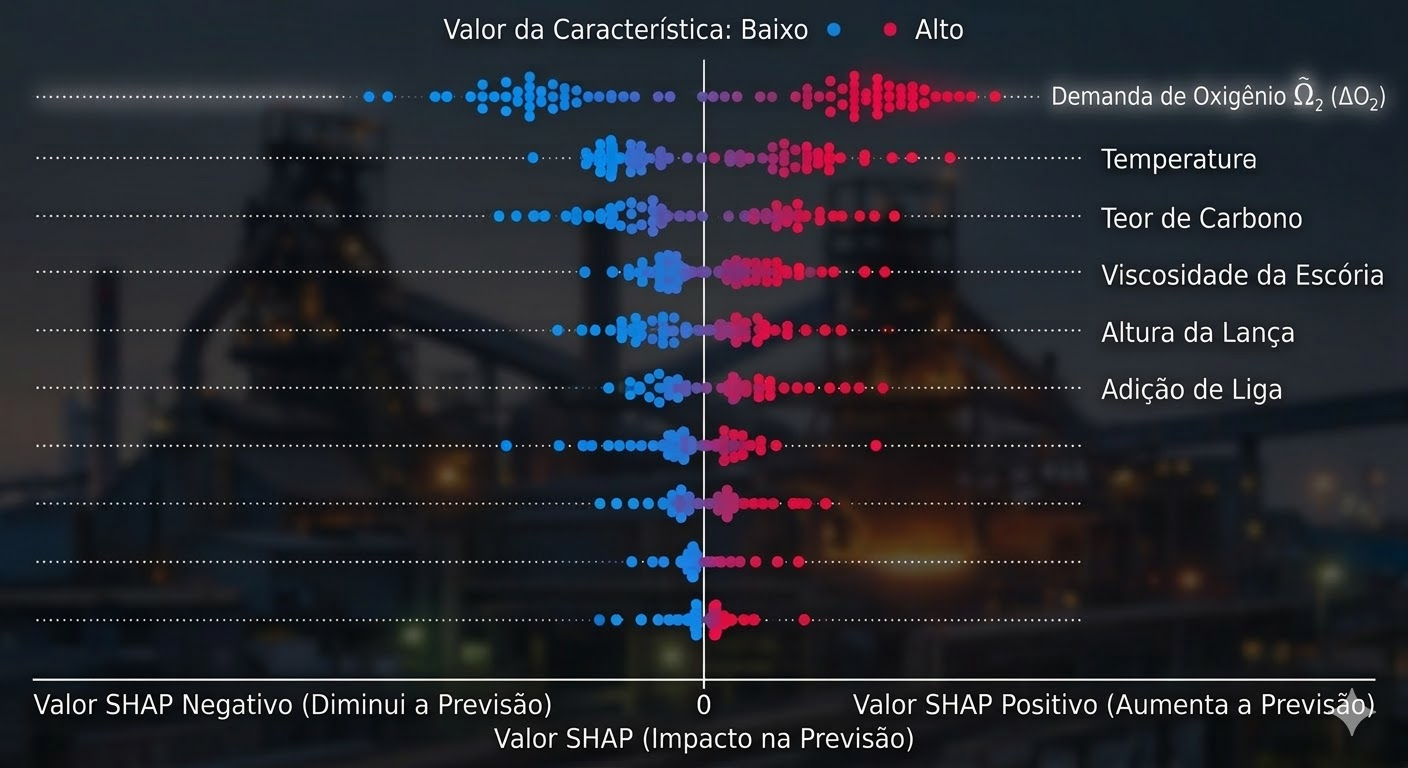
\includegraphics[width=0.65\textwidth]{Images/SHAP}
\caption{\textit{Beeswarm plot} SHAP conceitual: cada ponto representa a contribuição de um atributo para uma predição individual. Pontos à direita (vermelho) indicam impacto positivo na predição; à esquerda (azul), impacto negativo. A eficiência de consumo de O\textsubscript{2} (\texttt{o2\_efficiency}) é o atributo físico-derivado de maior importância para $[\text{C}]_\text{final}$ nos três modelos testados (Capítulo~\ref{chp:resultados}), em linha com o conhecimento metalúrgico de que a reação $\text{C} + \tfrac{1}{2}\text{O}_2 \rightarrow \text{CO}$ governa a descarburação. Ilustração gerada com auxílio de inteligência artificial (Nano Banana Pro~3).}
\label{fig:shap-beeswarm}
\end{figure}

\begin{figure}[H]
\centering
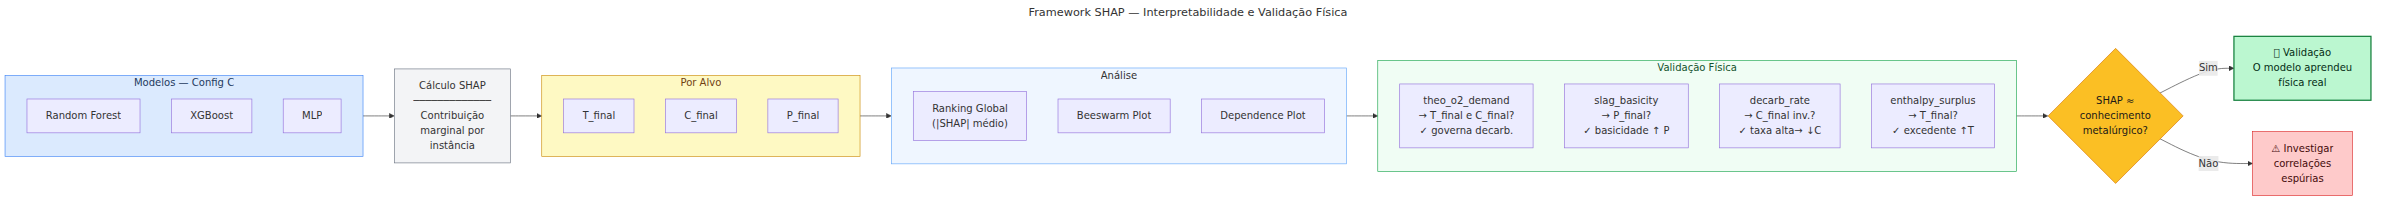
\includegraphics[width=0.88\textwidth]{Images/diagrams/06_shap_validation}
\caption{Framework de validação física por SHAP: os modelos treinados na Config~C são submetidos a análise SHAP por variável-alvo, gerando rankings de importância e gráficos de dependência. A consistência dos resultados com o conhecimento metalúrgico (\textit{e.g.}, basicidade da escória entre os atributos mais relevantes para P) é compatível com --- sem provar --- a captura de estrutura física pelo modelo; o Capítulo~\ref{chp:resultados} reporta que 4 das 5 hipóteses pré-registradas não foram falsificadas.}
\label{fig:shap-validation}
\end{figure}
